\chapter{传感原理与敏感元件}
\label{chap:sensing-principles}

\begin{focusbox}{本章复习路线}
传感器把力、位移、温度、光等被测量转换为可用信号。掌握一种传感器，不能只记住名称，还应能说明“\textbf{被测量先改变什么，随后检测什么，哪些因素也会改变输出}”。本章按下列链条组织：
\[
\text{被测量}\longrightarrow\text{敏感机理}
\longrightarrow\text{电参数或电信号}\longrightarrow\text{调理与读数}.
\]
\textbf{学习目标：}会计算应变片的微小电阻变化，比较电阻、电容和电感的测量电路；能解释光电、霍尔、光纤及常见机器人传感器的工作过程，并依据材料、频带、精度和环境条件选择测量方案。
\end{focusbox}

\begin{table}[H]
\centering\small
\begin{tabularx}{\linewidth}{@{}p{3cm} X@{}}
\toprule
复习模块 & 核心能力 \\
\midrule
电参数变化型 & 由 $\Delta R,\Delta C,\Delta L$ 推到电压、电流或频率变化。 \\
能量转换型 & 区分磁电、压电与热电的机理，识别静态、动态测量限制。 \\
光与磁敏感元件 & 分清内、外光电效应；用载流子受力解释霍尔电压。 \\
光纤与机器人传感 & 写出压力、位移、力触觉、测距和运动测量的转换链。 \\
检测与选型 & 说明裂纹检测方法的适用材料、缺陷位置与必要条件。 \\
\bottomrule
\end{tabularx}
\end{table}

\section{传感器的组成与分类}

\dfn{敏感元件与转换元件}{传感器感受规定的被测量，并按一定规律输出可用信号。\textbf{敏感元件}直接感受被测量，例如压力膜片；\textbf{转换元件}把其响应转换为便于传输、处理的信号，例如粘贴在膜片上的应变片。两者可能由不同零件完成，也可能合为一体。}

例如，应变式压力传感器的链条为
\[
p\longrightarrow\text{膜片变形}\longrightarrow\varepsilon
\longrightarrow\Delta R\longrightarrow U_o.
\]
最终测量的是压力，直接敏感的中间量却可能是应变。不同被测量可共用同一转换机理，同一被测量也可采用不同机理测量。

\begin{itemize}
\item \textbf{按被测量：}位移、速度、加速度、力、力矩、压力、温度、光强、磁场等。
\item \textbf{按工作原理：}电阻、电容、电感、磁电、压电、热电、光电、霍尔等。
\item \textbf{按信号变换特征：}物性型利用材料本身物理性质，如压电效应；结构型利用几何或结构参数，如极板间距改变电容。
\item \textbf{按能量关系：}能量转换型直接把被测对象输入的能量转换为信号，如磁电、压电和热电偶；能量控制型需外部激励，由被测量控制电参数或外部能量，如电阻应变片、电容与电感式传感器。
\end{itemize}

\nt{“有源、无源”在不同领域存在相反的命名习惯。判断时先说明\textbf{是否需要外部激励、信号能量来自哪里}，再给名称。能自行产生电荷或电动势的元件，其放大、显示电路仍可能需要供电。}

\textbf{弹性敏感元件：}梁、柱、膜片、膜盒、弹簧管和波纹管等将力或压力转换为变形。在线性弹性范围内可写 $F=kx$；结合材料关系 $\sigma=E\varepsilon$，就能把机械输入与应变、电容或电感联系起来。实际还须考虑蠕变、迟滞、温度和固有频率，避免只根据静态比例关系判断动态性能。

\Needspace{5cm}
\section{电阻式传感器：位移、应变与电阻变化}
\label{sec:ch4-resistance}
\noindent\keypoint{复习重点：$\Delta R/R=S_g\varepsilon$ 描述相对电阻变化；实际能否读出，还由测量电路和分辨力决定。}

\subsection{变阻器式与负载效应}
均匀导体满足
\[
R=\rho\frac{l}{A},
\]
其中 $\rho$ 为电阻率，$l$ 为长度，$A$ 为截面积。三者分别变化，都可能改变电阻。

变阻器式传感器用滑动触点改变有效电阻长度。设总长度 $l_p$、总电阻 $R_p$、触点位置 $x$，令 $\alpha=x/l_p\in[0,1]$；均匀电阻体的下段电阻 $R_x=\alpha R_p$。无负载时，以供电电压 $U_e$ 激励，输出为
\[
U_o=\frac{R_x}{R_p}U_e=\alpha U_e.
\]
若输出端接负载 $R_L$，下段变为 $R_x\parallel R_L$，则
\[
\boxed{\frac{U_o}{U_e}
=\frac{R_x\parallel R_L}{R_p-R_x+R_x\parallel R_L}
=\frac{\alpha}{1+(R_p/R_L)\alpha(1-\alpha)}}.
\]
有限负载使中间行程的输出低于理想直线，并引入非线性。增大后级输入电阻、采用缓冲器可减轻负载效应。滑动接触式结构简单，但受磨损、接触噪声和绕线节距限制；适合不要求极高分辨力的位移、角度等测量。

\subsection{金属应变效应与半导体压阻效应}
对电阻式取相对微分：
\[
\frac{\diff R}{R}=\frac{\diff\rho}{\rho}
+\frac{\diff l}{l}-\frac{\diff A}{A}.
\]
设导体沿轴向受小应变 $\varepsilon=\Delta l/l$，泊松比为 $\nu$，横向应变为 $-\nu\varepsilon$。忽略高阶项，有 $\Delta A/A\approx-2\nu\varepsilon$，于是
\[
\frac{\Delta R}{R}\approx(1+2\nu)\varepsilon
+\frac{\Delta\rho}{\rho}.
\]
\dfn{应变片灵敏度系数}{小应变线性范围内，定义
\[
\boxed{S_g=\frac{\Delta R/R}{\varepsilon}},\qquad
\boxed{\Delta R=RS_g\varepsilon}.
\]
$S_g$ 为无量纲量；$1\,\mu\varepsilon=10^{-6}$。应变的正负与所选方向有关，通常受拉为正、受压为负。}

金属应变片的几何尺寸变化占重要部分，电阻率变化也可有贡献，常用 $S_g$ 约为2；计算应采用给定或标定值，不能用某个泊松比随意替代。半导体应变片以\textbf{压阻效应}为主，电阻率随应力明显改变，灵敏度系数通常大得多，但温度影响、非线性与元件离散性也更明显。

\begin{table}[H]
\centering\small
\begin{tabularx}{\linewidth}{@{}l X X@{}}
\toprule
类型 & 主要特点 & 应用时关注 \\
\midrule
金属丝式、箔式 & 稳定性较好，便于粘贴和组成应变花；灵敏度系数较小。 & 粘贴质量、方向、温度补偿、导线电阻。 \\
半导体式 & 压阻效应显著，灵敏度高，尺寸小，易集成。 & 温漂、非线性、灵敏度离散性与机械强度。 \\
\bottomrule
\end{tabularx}
\end{table}

\subsection{从应变片到力、压力和加速度}
应变片需把被测应变传递到敏感栅上，因此粘贴层、方向和基体变形都会影响结果。用弹性体实现 $F\to\varepsilon$，可测力；用膜片实现 $p\to\varepsilon$，可测压力；用质量块的惯性力 $F\approx ma$ 作用于弹性体，可测加速度。线性近似还要求远离结构共振、变形不过大。

电桥能把微小电阻相对变化转换为接近零点的电压变化，便于差分放大。等臂单臂桥、小变化且输出近似开路时，
\[
\boxed{|U_o|\approx\frac{U_e}{4}\frac{|\Delta R|}{R}
=\frac{U_eS_g}{4}|\varepsilon|}.
\]
输出正负由桥臂位置及输出端极性决定；半桥、全桥可通过合理安排拉压应变提高灵敏度，并补偿某些共同温度影响。电桥仍需激励，且补偿效果取决于元件、温度与布置是否匹配。

\nt{\textbf{易错：}应变片并不直接输出“应变电压”，输出来自激励与电阻变化共同作用。$1000\,\mu\varepsilon=0.001$，不是 $1000$ 或 $0.001\%$；$\Delta R/R=0.002$ 对应 $0.2\%$。恒压供电时拉伸使 $R$ 增大、电流减小，电流相对变化与电阻相对变化只有在小量近似下互为相反数。}

\Needspace{5cm}
\section{电容式传感器：几何参数与介质变化}
\label{sec:ch4-capacitance}
\subsection{三类结构与灵敏度}
忽略边缘效应的平行板电容为
\[
\boxed{C=\frac{\varepsilon_0\varepsilon_rA}{\delta}},\qquad
\frac{\Delta C}{C}\approx\frac{\Delta\varepsilon_r}{\varepsilon_r}
+\frac{\Delta A}{A}-\frac{\Delta\delta}{\delta}.
\]
其中 $\varepsilon_0$ 为真空介电常数，$\varepsilon_r$ 为相对介电常数，$A$ 为有效相对面积，$\delta$ 为极距。这里 $\varepsilon_r$ 与机械应变 $\varepsilon$ 不同。

\begin{table}[H]
\centering\small
\begin{tabularx}{\linewidth}{@{}p{2.1cm} p{4.9cm} X@{}}
\toprule
变化参数 & 关系与特性 & 适用测量 \\
\midrule
变极距 & $C\propto1/\delta$，$\diff C/\diff\delta=-\varepsilon_0\varepsilon_rA/\delta^2$；灵敏度高但非线性。 & 微小位移、振动、膜片压力。 \\
变面积 & 固定极距、矩形重叠 $A=bx$ 时，$C=\varepsilon_0\varepsilon_rb x/\delta$，理想为线性。 & 较大直线位移、角位移。 \\
变介质 & 固定几何参数，$C$ 随介电常数或介质占据比例改变。 & 液位、材料厚度、湿度。 \\
\bottomrule
\end{tabularx}
\end{table}

变极距型若定义 $x>0$ 表示极距缩小，则
\[
C(x)=\frac{C_0}{1-x/\delta_0},\qquad
\frac{\Delta C}{C_0}=\frac{x/\delta_0}{1-x/\delta_0}
\approx\frac{x}{\delta_0}\quad(|x|\ll\delta_0).
\]
初始极距越小，位移灵敏度越高，但允许位移、过载裕量与防击穿要求会限制极距，不能无限缩小。

\subsection{差动电容：线性改善取决于读出量}
设中间动极板位移 $x$，两侧极距为 $\delta_0-x$、$\delta_0+x$，有效面积、介质相同，则
\[
C_1=\frac{C_0}{1-r},\quad C_2=\frac{C_0}{1+r},\quad r=\frac{x}{\delta_0},\quad |r|<1.
\]
电容差及其与电容和的比值分别为
\[
\frac{C_1-C_2}{C_0}=\frac{2r}{1-r^2}\approx2r,\qquad
\boxed{\frac{C_1-C_2}{C_1+C_2}=r=\frac{x}{\delta_0}}.
\]
差值消除了展开式中的偶次项，小位移灵敏度提高；若读出电容差与和的比值，在上述理想模型下可得到严格线性关系。寄生电容、边缘效应、极板不平行等仍会引入误差。

\begin{center}
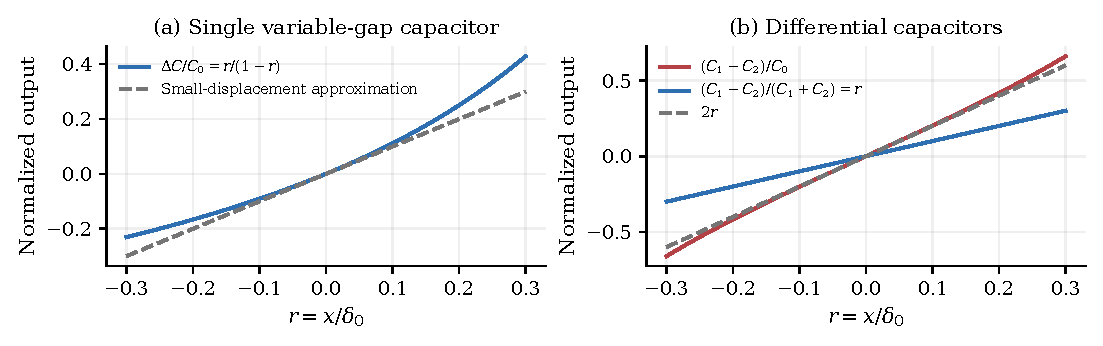
\includegraphics[width=.98\linewidth]{ch4-capacitance.pdf}
\end{center}
左图显示单电容的非线性；右图表明差动电容的“差值”与“差和比”是两个不同的读出量。

\subsection{测量电路与使用限制}
电容参数本身不能由直流电压表直接读出。可用交流电桥、阻抗分压、交流运算放大器、谐振或调频电路转换。若 $L$ 固定，LC振荡频率为
\[
f_0=\frac{1}{2\pi\sqrt{LC}},\qquad
\frac{\Delta f_0}{f_0}\approx-\frac12\frac{\Delta C}{C}.
\]
也可通过充放电时间或开关电容电路测量静态电容；直流极化方案适合某些动态电容变化。\textbf{静态被测量仍可用交流载波测出}，被测量变化频率与电路激励频率不是同一概念。

电容式传感器所需输入能量小、动态性能可较好，但电容量常小、输出阻抗高，电缆与邻近导体的寄生电容容易混入。短引线、屏蔽、保护环及前置电路可减轻影响；湿度、污染与介质变化也可能成为干扰。

\Needspace{5cm}
\section{电感式与涡流式传感器}
\label{sec:ch4-inductance}
\subsection{可变磁阻、自感与互感}
线圈自感可用磁路近似表示为
\[
\boxed{L\approx\frac{N^2}{\mathcal R_m}},\qquad
\mathcal R_m=\sum_i\frac{l_i}{\mu_i A_i},
\]
其中 $N$ 为匝数，$\mathcal R_m$ 为磁阻。若铁芯磁阻可忽略，磁路含两个相同气隙，每个长度为 $\delta$、截面积为 $A_0$，忽略漏磁与边缘效应，则
\[
L\approx\frac{N^2\mu_0 A_0}{2\delta}.
\]
改变气隙可获得高灵敏度的微位移测量，但 $L$ 对 $\delta$ 非线性；改变导磁面积或铁芯插入长度可扩大测量范围。采用差动结构可以提高中心附近灵敏度，并抵消部分共同影响。

\textbf{互感型：}一次线圈以交流激励，二次线圈的感应电压取决于互感。差动变压器利用两二次线圈反向串联，铁芯位于中心时输出近零，偏离中心后输出幅值反映位移大小，相对激励的相位反映方向。不能仅凭整流后的幅值判别正、负位移。

\subsection{涡流：导电体反作用于激励线圈}
交流线圈产生交变磁场；附近导电体中形成闭合涡流，涡流产生反作用磁场，并消耗能量，使线圈的等效电阻和电感改变。
\[
\boxed{Z_{\mathrm{coil}}=R_{\mathrm{eq}}+\iu\omega_eL_{\mathrm{eq}}
=Z(d,\rho,\mu,\omega_e,\text{几何形状})}.
\]
$d$ 为探头与工件间距，$\rho$ 为工件电阻率，$\mu$ 为磁导率，$\omega_e$ 为激励角频率。控制其他因素后，可由阻抗变化推断位移、振动、厚度或缺陷。

\textbf{裂纹为何能被检测？}裂纹阻断或绕转原有涡流路径，改变局部阻抗与损耗。裂纹方向与涡流方向、探头抬离距离、曲率和材料性质都会影响信号，应通过扫描和参考试样区分这些影响。

导电体中的趋肤深度近似为
\[
\delta_s=\sqrt{\frac{2\rho}{\omega_e\mu}}
=\frac{1}{\sqrt{\pi f_e\mu\sigma_e}},
\]
其中 $\sigma_e=1/\rho$ 为电导率。频率升高时，电流更集中于表层，利于表面或近表面缺陷检测；频率降低可增加穿透，但探测深度、分辨力与信噪比还受材料和结构限制。

\nt{涡流检测要求被测区域具有足够导电性，\textbf{不要求一定是铁磁性材料}；非导电陶瓷通常不能直接采用常规涡流检测。高频反射、低频透射是常见配置，不应把某个固定频率界限当作所有材料的通用界限。涡流元件的输出是激励线圈阻抗的变化，不等同于无需激励的磁电发电式元件。}

\subsection{测量电路}
自感和涡流元件常用交流电桥或阻抗分压，将 $\Delta L$、$\Delta R_{\mathrm{eq}}$ 转为载波幅值、相位变化，再解调；也可放入振荡器，用频率变化读出。若只变 $L$，
\[
\frac{\Delta f_0}{f_0}\approx-\frac12\frac{\Delta L}{L}.
\]
与电容式相比，电感式需特别关注线圈电阻、磁芯非线性、磁滞、漏磁、外部磁场及导体材质变化。元件“结构简单”并不意味着输出只受位移影响。

\Needspace{5cm}
\section{磁电、压电与温度传感}
\label{sec:ch4-generating}
\subsection{磁电式：变化磁通产生电动势}
\dfn{电磁感应转换}{线圈的感应电动势为
\[
\boxed{e=-N\frac{\diff\Phi}{\diff t}},\qquad
\Phi=\int\mathbf B\cdot\diff\mathbf S.
\]
在均匀磁场、直导线有效长度 $l$、运动方向与磁场和导线均垂直时，电动势大小为 $|e|=Bl|v|$。}

动圈式振动速度传感器用线圈与磁体之间的相对运动产生信号；转速传感器可利用齿轮运动引起磁路磁通周期变化。测得的是\textbf{磁通变化率}或相关运动量。恒定磁通不产生感应电动势，因此不能把磁电感应式当成直接测静态磁场或静态位移的元件。

\subsection{压电式：应力产生极化电荷}
\dfn{正、逆压电效应}{正压电效应指某些材料受力后发生极化，在表面产生电荷；逆压电效应指施加电场后材料产生机械变形。传感接收主要利用正效应，超声发射等执行过程利用逆效应。}

在给定受力方向和电极配置下，可用
\[
\boxed{Q=d_FF},\qquad U_{\mathrm{oc}}\approx\frac{Q}{C_p}
\]
描述，其中 $d_F$ 为该结构下的电荷灵敏度（$\mathrm{C/N}$），$C_p$ 为元件电容。常见材料包括石英等单晶、压电陶瓷以及PVDF压电薄膜。

实际压电元件可近似为电荷源与电容、漏电阻并联；电缆与放大器也引入电容和漏电。恒定力产生的初始电荷会逐渐泄漏，使读数随时间衰减。若等效时间常数为 $\tau=R_{\mathrm{eq}}C_{\mathrm{eq}}$，简单模型的归一化动态关系为
\[
H_p(s)=\frac{s\tau}{1+s\tau},\qquad
|H_p(\iu\omega)|=\frac{\omega\tau}{\sqrt{1+(\omega\tau)^2}}.
\]
故压电式通常适合振动、冲击、动态力和加速度测量；准静态能力取决于时间常数与测量持续时间，不能笼统宣称能长期测恒定力。

\textbf{电压读出与电荷读出：}电压放大器读出的电压易受元件、电缆及输入电容影响；电荷放大器在理想工作频带内近似有 $U_o=-Q/C_f$，由反馈电容 $C_f$ 决定增益，并减轻电缆电容对电荷增益的影响。实际低频下限还受反馈电阻、漏电与漂移限制。

若两个相同压电片各产生电荷 $q$、电容 $C_p$，且受力与极性配置能使输出相加，则串联等效电容 $C_p/2$、开路电压 $2q/C_p$；并联等效电容 $2C_p$、总电荷 $2q$、开路电压 $q/C_p$。\textbf{串联增大电压，并联增大电荷；时间常数还取决于所接电路，不能仅由串并联方式决定。}

\subsection{温度测量：热电偶、热电阻与辐射}
\begin{table}[H]
\centering\small
\begin{tabularx}{\linewidth}{@{}p{2.2cm} X X@{}}
\toprule
方法 & 敏感关系 & 主要限制 \\
\midrule
热电阻 & 金属电阻随温度改变，局部近似 $R(T)\approx R(T_0)[1+\alpha(T-T_0)]$。 & 需激励；导线电阻、自热与热惯性影响读数。 \\
热敏电阻 & 半导体电阻随温度显著变化；常见NTC随温度升高而阻值减小。 & 灵敏度高，但非线性强，须标定或线性化。 \\
热电偶 & 两种不同导体组成回路，测量端与参考端温度不同而产生热电势。 & 输出取决于温差及材料，需参考端补偿；热惯性、安装导热也有影响。 \\
辐射测温 & 由目标热辐射的强度或光谱推断温度，非接触。 & 发射率、反射背景、光路透过率与视场影响结果。 \\
\bottomrule
\end{tabularx}
\end{table}

热电偶电势可表示为 $E=\int_{T_r}^{T_h}[S_A(T)-S_B(T)]\diff T$，$T_h$、$T_r$ 分别为测量端与参考端温度。接触式测温依靠热交换达到接近热平衡，可能改变局部温度场且存在响应延迟；非接触式省去接触，却需建立辐射与温度间的可靠关系。测温范围与精度须按具体材料和结构确认。

\Needspace{5cm}
\section{光电传感器：效应、读出与光路}
\label{sec:ch4-photoelectric}
\noindent\keypoint{复习重点：外光电效应的电子逸出材料表面；内光电效应发生在材料内部，包含光导与光生伏特两类。}

\subsection{按物理效应分类}
\begin{table}[H]
\centering\small
\begin{tabularx}{\linewidth}{@{}p{2.2cm} X X@{}}
\toprule
效应与元件 & 工作过程 & 特点与读出 \\
\midrule
外光电效应：光电管、光电倍增管 & 入射光使光阴极电子逸出表面，阳极收集电子；倍增管还用倍增极实现二次电子倍增。 & 可用于微弱光检测；倍增管通常需高压，体积与供电要求较高。 \\
内光电效应：光导型 & 光照增加可参与导电的载流子，改变材料电导率，如光敏电阻。 & 需外部激励，通常照度越强电阻越低；响应速度、线性、暗电阻和温度效应取决于材料。 \\
内光电效应：光生伏特型 & 光生电子、空穴被结区内建电场分离，产生光电流或光电压，如光电池、光伏模式光电二极管。 & 可在零外加偏压下检测光；适合光强、光功率等测量。 \\
\bottomrule
\end{tabularx}
\end{table}

光电二极管也可反向偏置运行，常称光导模式，可减小结电容、提高带宽；此时须考虑暗电流和噪声。因此\textbf{元件名称、物理效应与偏置方式应分别说明}，不能把所有半导体光电器件都当成光敏电阻。

在给定波长、线性范围内，光电二极管可近似有 $I_{\mathrm{ph}}=\mathcal R_\lambda P$，$P$ 为入射光功率，$\mathcal R_\lambda$ 为光谱响应度（$\mathrm{A/W}$）。响应度随波长而变，选择元件时需使光源波段与探测器光谱响应匹配。

\subsection{被测量如何调制光}
\begin{enumerate}
\item \textbf{自辐射：}目标本身发光或辐射，光信号携带目标温度、辐射强度等信息。
\item \textbf{吸收或透射：}被测物改变透射光强或光谱，可测浓度、透明度、浑浊度及介质厚度。
\item \textbf{反射：}表面位移、粗糙度、颜色或缺陷改变接收光强及其空间分布。
\item \textbf{遮光或光束位置变化：}物体位置改变光通量或光斑位置，可测尺寸、位移、振动、转角，并实现计数、测速。
\end{enumerate}

\textbf{模拟式与脉冲式：}模拟式依据光电流或电压连续变化量测量，较关注线性、漂移和背景光；脉冲式通过阈值把明暗变化变为通断脉冲，适合计数和编码，但阈值、对比度、响应时间与误触发同样重要。

\ex{由遮光脉冲计算转速}{转盘每周有 $z$ 个等间距透光窗，检测到脉冲频率 $f_p$。若每窗只计一次且无漏计，则每秒转数为 $f_p/z$，转速为
\[
n=\frac{60f_p}{z}\quad(\mathrm{r/min}).
\]
脉冲电平幅值主要保证可靠识别，转速由脉冲\textbf{频率}而非幅值给出。}

\nt{一种反射式光电探头的强度变化可能同时来自位移、目标反射率和光源漂移。只有在光路、目标表面及光源条件受控或经过补偿时，才能把强度稳定换算成位移。光电检测可非接触，但并非天然不受环境光、污染或遮挡影响。}

\Needspace{5cm}
\section{霍尔效应与磁场相关测量}
\label{sec:ch4-hall}
\dfn{霍尔效应}{在导体或半导体薄片中通入电流，若施加垂直于电流的磁场，载流子受洛伦兹力发生横向偏转，在同时垂直于电流和磁场的方向建立电场与电压，这一现象称为霍尔效应。}

\subsection{物理本质与电压关系}
设电流沿 $x$ 方向，磁场沿 $z$ 方向，霍尔电压在 $y$ 方向测量；薄片宽度为 $w$，沿磁场方向的厚度为 $t$。载流子平均漂移速度为 $\mathbf v_d$，电荷为 $q$，磁力为 $q\mathbf v_d\times\mathbf B$。横向电荷积累产生电场，稳态满足
\[
q(\mathbf E_H+\mathbf v_d\times\mathbf B)=0.
\]
这说明霍尔效应的本质是\textbf{运动载流子在磁场中受力、横向电荷分离，直到电场力与磁力平衡}。

对均匀材料、单一主导载流子、简单低场模型，用大小关系 $|I_b|=n|q|v_dwt$、$|E_H|=v_d|B_\perp|$，得到
\[
|U_H|=|E_H|w=\frac{|I_bB_\perp|}{n|q|t}.
\]
考虑材料与几何系数，常写为
\[
\boxed{U_H=K_HI_bB_\perp},\qquad
K_H\approx\frac{R_H}{t},\quad R_H=\frac{1}{nq}.
\]
$I_b$ 为霍尔元件的偏置电流，$B_\perp$ 为垂直薄片的磁感应强度分量；电压符号还取决于载流子类型与端子方向。反转偏置电流或磁场中的一个，理想霍尔电压反号；两者同时反转，则符号不变。

\subsection{三类典型应用}
\begin{enumerate}
\item \textbf{磁场测量：}恒定 $I_b$，由 $U_H$ 推算 $B_\perp$。霍尔元件能测静态磁场，这与依赖磁通变化的感应线圈不同。
\item \textbf{电流测量：}被测导线电流 $I_m$ 产生磁场，使 $B\propto I_m$，再由霍尔电压反推电流；磁芯气隙结构可集中磁通。注意 $I_m$ 与元件偏置电流 $I_b$ 是两个不同电流。
\item \textbf{位移、转角或转速测量：}磁体与霍尔元件相对运动使 $B$ 改变。标定 $B(x)$ 可测位移；测磁场矢量方向可测角度；识别每周磁极经过产生的脉冲，可由脉冲频率计算转速。
\end{enumerate}

霍尔本身直接敏感磁场，其他量都需经过“被测量 $\to B\to U_H$”的结构变换。位移与磁场通常非线性；温度、零点偏置、外部磁场、磁体特性和安装气隙都会影响测量。闭环、差动或补偿结构可改善部分误差，但仍须标定。

\nt{\textbf{易错：}霍尔电压并非电磁感应电动势，不要求磁场随时间变化；它也不是磁阻效应。公式中的 $B_\perp$ 必须取对敏感面的法向分量，磁场平行于普通平面霍尔元件敏感面时，该分量为零。}

\Needspace{5cm}
\section{光纤传感器：光学调制与机械转换}
\label{sec:ch4-fiber}
\subsection{光纤是传输介质，也可以是敏感元件}
光纤传感器通过被测量改变光的\textbf{强度、相位、波长、频率或偏振态}，再检测该变化。
\begin{itemize}
\item \textbf{传光型：}光纤主要负责引导光，被测量作用于光纤外的反射面、膜片、遮光片或光学腔。
\item \textbf{传感型：}光纤本身参与敏感，如应变或温度改变光纤折射率、长度或光栅周期。
\end{itemize}
光纤具有电绝缘、抗电磁干扰、可远距离传输和易于多点布置等优点；但“光纤传感”并不必然是非接触测量，粘贴在结构上的光纤应变计就是接触式测量。

\subsection{反射强度式压力与位移测量}
\textbf{位移测量：}发射光纤把光照向目标，接收光纤收集反射光。目标与探头间距 $d$ 改变光斑扩展、重叠区域及耦合效率，得到
\[
P_r=P_t\eta(d),\qquad U_o\propto P_r.
\]
$P_t,P_r$ 为发射与接收光功率，$\eta(d)$ 为含光路几何与反射率的耦合系数。标定后在\textbf{单调工作区间}内由输出求位移；强度与距离通常不是全量程单调或线性的。

\textbf{压力测量：}压力先作用于弹性膜片，使膜片产生位移 $x_d$，反射面的间距随之改变，再按上述光强耦合机理读出。在线性弹性范围内可近似写
\[
p\longrightarrow x_d=k_pp
\longrightarrow\eta(d_0-x_d)\longrightarrow P_r\longrightarrow U_o.
\]
两者可共用光学读出，\textbf{差别在于压力测量多了一次“压力 $\to$ 弹性变形”的机械变换}，标定关系还由膜片刚度、有效面积、预紧与温度决定。

\begin{center}
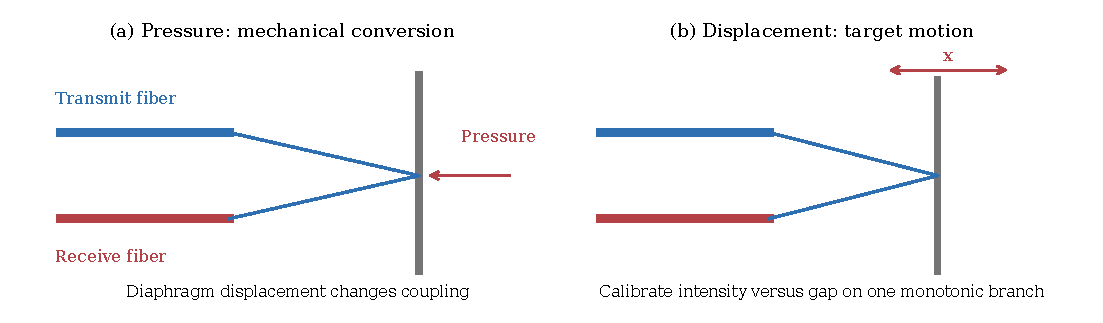
\includegraphics[width=.98\linewidth]{ch4-fiber-pressure-displacement.pdf}
\end{center}
左图由压力驱动膜片反射面，右图由目标自身位移改变间距；箭头表示一种选定的运动方向，输出增减还需依据实际光强标定曲线判断。

\subsection{光纤光栅与相位型测量}
光纤布拉格光栅（FBG）反射特定波长，中心波长为
\[
\boxed{\lambda_B=2n_{\mathrm{eff}}\Lambda},\qquad
\frac{\Delta\lambda_B}{\lambda_B}
\approx\frac{\Delta n_{\mathrm{eff}}}{n_{\mathrm{eff}}}
+\frac{\Delta\Lambda}{\Lambda}.
\]
$n_{\mathrm{eff}}$ 为有效折射率，$\Lambda$ 为光栅周期。轴向应变既改变周期，也通过弹光效应改变折射率；温度同样影响两者，常以
\[
\frac{\Delta\lambda_B}{\lambda_B}=K_\varepsilon\varepsilon+K_T\Delta T
\]
表示小变化关系。测力、压力时需由弹性结构把载荷传递为光纤应变，并补偿温度交叉敏感。波长读出对单纯光强波动较不敏感，但不等于无漂移。

相位型则利用光程变化，例如光学腔长度 $d$ 改变引起往返相位变化 $\Delta\phi=4\pi n\Delta d/\lambda$（$\lambda$ 为真空波长，折射率 $n$ 固定）。因此不能把“压力一定调相位、位移一定调强度”当成定义；两种被测量都可采用强度、相位或波长读出，关键是具体结构的转换链。

\Needspace{5cm}
\section{机器人中的力触觉、测距与运动传感}
\label{sec:ch4-robot-sensing}
\subsection{力与触觉：从集中载荷到分布接触}
单维力传感器给出一个力分量；六维力/力矩传感器通过弹性体上多组敏感元件与标定解耦，估计 $F_x,F_y,F_z,M_x,M_y,M_z$。力与力矩量纲不同，六个通道也不能简单相加。

\begin{table}[H]
\centering\small
\begin{tabularx}{\linewidth}{@{}p{2.1cm} X X@{}}
\toprule
触觉方案 & 主要转换链 & 测量特点 \\
\midrule
电阻/压阻式 & 接触载荷 $\to$ 材料电阻率或导电接触网络变化 $\to\Delta R$。 & 可测静态接触；关注迟滞、蠕变、温漂。 \\
电容式 & 压力 $\to$ 柔性介质或极板变形 $\to\Delta C$。 & 适合小力和分布接触；关注寄生电容与结构耦合。 \\
压电式 & 动态接触力 $\to$ 极化电荷。 & 适合冲击、滑移或振动；长期静态力受漏电影响。 \\
光纤光栅式 & 力 $\to$ 弹性体与光纤应变 $\to\Delta\lambda_B$。 & 可多点布置、抗电磁干扰；需温度补偿。 \\
视触觉 & 接触使弹性表面变形 $\to$ 内部光照与相机图像 $\to$ 形状和接触量估计。 & 可提供较丰富的空间接触信息；依赖光学结构、材料模型与标定。 \\
\bottomrule
\end{tabularx}
\end{table}

触觉阵列强调接触\textbf{位置与分布}，力/力矩传感器强调载荷合量。二者可互补；空间分辨力高并不自动意味着力测量准确度高。

\subsection{测距：时间、相位与三角几何}
\dfn{往返飞行时间法}{信号从传感器传播到目标并返回，传播速度 $v$ 已知、往返时间为 $\Delta t$，则
\[
\boxed{d=\frac{v\Delta t}{2}},\qquad
\Delta d\approx\frac{v}{2}\Delta(\Delta t).
\]
光在空气中可近似取 $v\approx3.0\times10^8\,\mathrm{m/s}$；超声的声速应按介质与温度确定，室温空气中约 $340\,\mathrm{m/s}$。单程计时或到达时间差定位需另建模型，不能一律除以2。}

光测距的时间分辨要求很高：$1\,\mathrm{mm}$ 的距离变化对应约 $6.67\,\mathrm{ps}$ 的往返时间变化。超声传播慢，计时较容易，但温度、气流、近场盲区、目标倾斜、吸声及多径会影响结果。

连续调制光测距用\textbf{调制包络}的往返相位差。若调制频率 $f_m$、传播速度 $c$，则
\[
\boxed{d=\frac{c\Delta\phi}{4\pi f_m}},\qquad
0\leq\Delta\phi<2\pi.
\]
相位以弧度代入；不含整数周信息时，无模糊距离为 $c/(2f_m)$。这里的波长 $c/f_m$ 是调制波长，不能用光载波波长代替。多频或其他先验信息可用于解模糊。

三角测量使用光源、目标与接收器之间的基线及视角几何。某一理想几何下可写 $d=ab/x$，$a$ 为基线、$b$ 为接收光学参数、$x$ 为像面光斑偏移；具体式子由标定坐标决定。若 $a,b$ 固定，
\[
|\Delta d|\approx\frac{ab}{x^2}|\Delta x|
=\frac{d^2}{ab}|\Delta x|,
\]
说明像面分辨力固定时，距离越远，距离分辨力通常越差。

\begin{table}[H]
\centering\small
\begin{tabularx}{\linewidth}{@{}p{2.2cm} X X@{}}
\toprule
方案 & 主要信息与原理 & 适用条件与限制 \\
\midrule
激光雷达 & 测距加扫描或多通道采样，形成角度与距离信息及点云。 & 角分辨力、视场、刷新率和量程共同决定空间采样；受目标反射、遮挡与环境影响。 \\
ToF相机 & 在图像阵列各像素测往返时间或调制相位，得到深度图。 & 关注像素混合、多径、背景光与同步干扰。 \\
结构光 & 投射已知图案，识别图案与像素对应关系，由三角几何求深度。 & 依赖标定与图案可见性；反光、遮挡、强背景光可能破坏匹配。 \\
超声 & 压电换能器发射、接收声波，以时间或幅度等检测目标。 & 可用于透明物体和部分低能见度场景；声速与反射条件影响测量。 \\
毫米波雷达 & 利用电磁波传播、反射与多普勒信息测距离、速度等。 & 可在部分恶劣天气下保持探测能力；分辨力取决于带宽、天线与处理方法。 \\
\bottomrule
\end{tabularx}
\end{table}

\nt{传感器之间不存在脱离条件的统一精度排序。选择激光、超声或雷达，应针对量程、空间分辨力、目标材质、环境、刷新率与成本比较。光传播快也不表示整个测量系统必然有更低延迟，采样、扫描和处理时间同样计入。}

\subsection{光栅、编码器与速度}
光栅通过均匀条纹与光电检测把位移转换为周期信号。两光栅小角度相交可形成莫尔条纹，将微小位移表现为较宽条纹的移动。若栅距为 $W$，每栅距产生一个计数，则 $x=NW$；若每栅距细分为 $q$ 个计数，则
\[
x=\frac{N_cW}{q},
\]
$N_c$ 为实际累计计数。刻线密度影响可获得的分辨力，但实际准确度还取决于刻线、安装、细分与读数误差。

\textbf{绝对式编码器：}每个角位置对应一个码字。$n_b$ 位理想单圈编码器可区分 $2^{n_b}$ 个位置，角分辨力为 $360^\circ/2^{n_b}$。普通二进制跨边界时可能多位同时变化；格雷码相邻码字只变一位，能降低不同步读数产生的大幅跳变。

\textbf{增量式编码器：}用周期脉冲累计相对位移，用A、B两相正交信号辨向，Z相信号提供每周参考。若每周每相有 $N$ 个周期，采用 $q$ 倍计数，则
\[
\boxed{\Delta\theta=\frac{360^\circ}{qN}},\qquad
\boxed{n=\frac{60f_c}{qN}\quad(\mathrm{r/min})},
\]
$f_c$ 为按同样规则得到的\textbf{计数事件率}；若用A相周期频率则分母为 $N$。丢失计数会累积位置误差，重新上电后一般需寻找参考。

\begin{center}
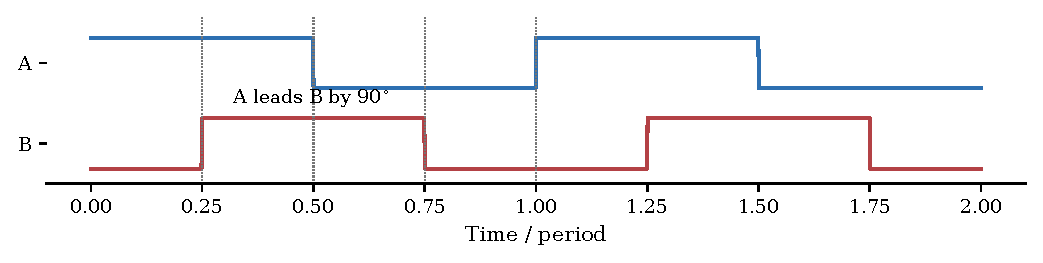
\includegraphics[width=.88\linewidth]{ch4-encoder.pdf}
\end{center}
图示A超前B $90^\circ$ 的一种方向；反转时先后关系交换。四倍计数利用两相的上升、下降沿，不能把“每相周期数”和“每周计数数”混用。

\subsection{加速度、角速度与姿态}
加速度计常用质量块、弹性支承及位移或力敏感元件。在线性、低于固有频率的适用区，可用惯性力 $F\approx ma$ 关联电容、电阻或压电输出。加速度计测得的是比力，静止时仍能感受到重力相关输出；将其积分求速度、位移时，偏置会积累为漂移。

陀螺仪测角速度。机械陀螺利用角动量与进动；MEMS陀螺常利用振动质量的科里奥利耦合；光学陀螺利用旋转导致的光程相位差。三轴陀螺与三轴加速度计组成常见六轴IMU，加入三轴磁力计常称九轴组合。\textbf{姿态是由这些量与模型融合估计的结果}，不能把IMU简单等同于无漂移的三轴角度计。磁力计提供磁场方向相关信息，但会受环境磁场干扰。

速度还可由位移差分、加速度积分或多普勒频移获得。单基地往返测量、速度远小于波速时，$f_D\approx2v_r/\lambda$，$v_r$ 为径向速度；该关系说明频移与速度成正比、与波长成反比。非径向运动需取速度在视线方向的投影。

\Needspace{5cm}
\section{传感器的选用原则}
\label{sec:ch4-selection}
选择传感器应先把测量任务写清楚：被测量及其范围、最小待测变化、变化频率、允许误差、安装方式和环境条件。随后检查机理是否可行，再比较具体性能。

\begin{enumerate}
\item \textbf{量程、灵敏度与分辨力：}最大输入不能导致饱和或损坏，最小变化应能超过噪声、漂移和读数分辨力。提高灵敏度可能缩小量程，也会放大干扰。
\item \textbf{响应与工作频带：}在被测信号占据的频带内检查幅值与相位，必要时用第3章的一阶、二阶模型计算误差；不要只看标称带宽或固有频率。
\item \textbf{线性范围与静态误差：}检查非线性、回程、重复性、零漂、温漂和交叉敏感，明确是否需补偿与标定。
\item \textbf{测量方法与对象：}决定接触或非接触、在线或离线；考虑材料导电性、磁性、光学反射、声学耦合及被测对象是否允许被加载。
\item \textbf{可靠性与环境：}在规定温度、湿度、振动、污染及电磁环境中能否持续完成测量，安装与电缆是否引入附加误差。
\item \textbf{系统配套与经济性：}激励、放大器、解调器、采样接口与传输方式应匹配，兼顾体积、质量、价格、维护、更换与长期标定成本。
\end{enumerate}

\begin{focusbox}{选型结论要形成闭合的证据链}
\[
\text{任务要求}\longrightarrow\text{候选机理与适用条件}
\longrightarrow\text{量程、分辨力和频带核查}
\longrightarrow\text{干扰及校准措施}.
\]
例如“选涡流检测裂纹”的结论还应交代材料导电、缺陷位于可探测深度、探头可接近、抬离与材质影响可校准。能够列出元件名称，只完成了选型的第一步。
\end{focusbox}
